\documentclass[10pt,a4paper,onecolumn]{article}

\usepackage[utf8]{inputenx}
\usepackage[T1]{fontenc}
\usepackage{lmodern}
\usepackage{listings}
\usepackage{textcomp}
\usepackage[english,italian]{babel}
\usepackage{amsmath}
\usepackage{booktabs}
\usepackage{graphicx}
\usepackage[font=small,labelfont=bf,labelsep=period,tableposition=top]{caption}
\usepackage{tabularx}
\usepackage{multirow}
\usepackage{booktabs}
\usepackage{longtable}
\usepackage{fancyhdr}
\usepackage{lastpage}    
\usepackage{color}

\fancyhead{}
\renewcommand{\headrulewidth}{1pt}

\fancyhead[RE,RO]{
\begin{picture}(-135,0)
	%TODO \put(-482,-14){\includegraphics[width=0.26\textwidth]{logoHead.png}} non sono molto bravo con gli strumenti grafici... qualcuno può creare un mini logo da collocare in questa posizione... l'idea è fare la scritta "Progetto di TecWeb... magari a destra di un simbolo che possa rappresentare internet... come... booo.. un mondo con un a rete attorno.... oppure un agglomerato dei loghi di browser come quella che ho scaricato!
	\put(-475,0){\sffamily\large\leftmark}
\end{picture}
}

\cfoot{}

\fancyfoot[RO,LE]{\sffamily Pag.~\thepage{} di \pageref{LastPage}} 
\fancyfoot[RE,LO]{Il mondo di Babe}

\renewcommand{\footrulewidth}{.2pt}
\pagestyle{fancy}

\renewcommand{\sectionmark}[1]{\markboth{#1}{#1}} 

% **************************************************
% Cross-references e collegamenti ipertestuali
% **************************************************
\usepackage[hidelinks]{hyperref}
\hypersetup{%
  colorlinks=false, linktocpage=false, pdfborder={0,0,0}, pdfstartpage=1, pdfstartview=FitV,%
  urlcolor=Cyan, linkcolor=Cyan, citecolor=Black, %pagecolor=Black,
  pdfcreator={pdflatex}, pdfproducer={pdflatex with hyperref package}%
}

\definecolor{dkgreen}{rgb}{0,0.6,0}
\definecolor{gray}{rgb}{0.5,0.5,0.5}
\definecolor{mauve}{rgb}{0.58,0,0.82}
 
\lstset{ %
  language=java,                % the language of the code
  basicstyle=\footnotesize,           % the size of the fonts that are used for the code
  numbers=left,                   % where to put the line-numbers
  numberstyle=\tiny\color{gray},  % the style that is used for the line-numbers
  stepnumber=2,                   % the step between two line-numbers. If it's 1, each line 
                                  % will be numbered
  numbersep=5pt,                  % how far the line-numbers are from the code
  backgroundcolor=\color{white},      % choose the background color. You must add \usepackage{color}
  showspaces=false,               % show spaces adding particular underscores
  showstringspaces=false,         % underline spaces within strings
  showtabs=false,                 % show tabs within strings adding particular underscores
  frame=single,                   % adds a frame around the code
  rulecolor=\color{black},        % if not set, the frame-color may be changed on line-breaks within not-black text (e.g. comments (green here))
  tabsize=2,                      % sets default tabsize to 2 spaces
  captionpos=b,                   % sets the caption-position to bottom
  breaklines=true,                % sets automatic line breaking
  breakatwhitespace=false,        % sets if automatic breaks should only happen at whitespace
  title=\lstname,                   % show the filename of files included with \lstinputlisting;
                                  % also try caption instead of title
  keywordstyle=\color{blue},          % keyword style
  commentstyle=\color{dkgreen},       % comment style
  stringstyle=\color{mauve},         % string literal style
  escapeinside={\%*}{*)},            % if you want to add LaTeX within your code
  morekeywords={*,...},              % if you want to add more keywords to the set
  deletekeywords={...}              % if you want to delete keywords from the given language
}

% **************************************************
% Macro
% **************************************************
\newcommand{\sitepage}[1]{\textsf{``#1''}}
\newcommand{\inglese}[1]{\foreignlanguage{english}{\itshape{}#1}}

\begin{document}
%----------------------------------------------------------
\begin{titlepage}

\begin{center}
% Upper part of the page
 
\textsc{\Large}\\[5cm]

\includegraphics[width=0.4\textwidth]{Logo.png}\\[0.3cm]  
\noindent\rule{\textwidth}{0.4pt} \\[0.3cm]
\textsc{\Huge Progetto di}\\[0.25cm]
\textsc{\Huge Tecnologie Web}\\[0.3cm]
\textsc{\Large Sito ``Il mondo di Babe''}
\noindent\rule{\textwidth}{0.4pt}\\[0.5cm]
\textit{``Sviluppare un sito accessibile secondo gli standard web''} \\[0.5cm]
\textsc{20 febbraio 2013}\\[0.5cm]
\begin{minipage}{0.4\textwidth}
\begin{flushleft} \large
\emph{Studente:}\\
Andrea Meneghinello\\
Andrea Rizzi\\
Diego Beraldin\\
Elena Zecchinato
\end{flushleft}
\end{minipage}
\begin{minipage}{0.4\textwidth}
\begin{flushright} \large
\emph{Matricola:} \\
610762\\
610761\\
booo\\
booo\\
\end{flushright}
\end{minipage}
\end{center}
\end{titlepage}
%-----------------------------------------------------------------------

\clearpage

\tableofcontents

\clearpage 

\begin{abstract}

\end{abstract}

\clearpage

\section{Analisi dei requisiti}
% chi sono i destinatari del sito, quali sono le loro necessita' e come le soddisfiamo
% font, colori, immagini

\section{Progettazione architetturale}
% quale schema organizzativo e' stato scelto, come sono state organizzate le informazioni

\section{Mappa del sito}
\begin{figure}[tb]
\centering
\includegraphics[width=.8\textwidth]{mappasito.png}
\caption{Organizzazione delle pagine del sito}
\end{figure}

\clearpage

\section{Accessibilità}

\subsubsection{Collegamenti}
Per rendere più rapida la navigazione si è scelto di offrire la possibilità di saltare gli elementi che esulano dal contenuto in senso stretto, quali il menu di navigazione o la lista dei \inglese{feed RSS} che si ripetono uguali in ogni pagina e che dunque non necessitano di essere letti ogni volta. A tal fine, sono stati inseriti dei collegamenti nascosti (impostando una posizione assoluta che ecceda il margine sinistro), che però risultano accessibili se si legge il solo contenuto testuale della pagina.

Si è inoltre prestata particolare attenzione a evitare la presenza di link circolari, a rendere il testo delle ancore facilmente individuabile e, soprattutto, sufficientemente autoesplicativo riguardo alla posizione di destinazione (evitando accuratamente di utilizzare parole ``vuote'' o deittici come testo dei link).

Le pagine di dimensione verticale maggiore, ad esempio \sitepage{Alfabeto}, \sitepage{Mesi} o \sitepage{Trama} contengono inoltre dei collegamenti interni per tornare in cima alla pagina durante la navigazione. La pagina dei \sitepage{Personaggi}, oltre a questo tipo di collegamenti, permette di spostarsi da un personaggio all'altro durante la lettura.

La presenza di link esterni al sito, infine, è stata resa evidente mediante l'utilizzo di una simbologia esplicita e tale convenzione interna è stata mantenuta per tutte le pagine.
%TODO specificare dove esattamente sono stati riportati i link esterni

\subsection{Tabelle}
Le tabelle che compaiono nella sezione \sitepage{Interpreti} sono state progettate per essere fruibili anche in forma non visuale, mediante l'utilizzo dell'attributo \texttt{scope} rispettivamente con il valore \texttt{col} per le intestazioni delle colonne e con il valore \texttt{row} per la testata di ogni riga, ovvero il personaggio di cui si elencano gli attori della versione originale e i doppiatori della versione italiana.

La disposizione delle informazioni nella tabella è resa ancor più chiara dall'attributo \texttt{summary}, in cui oltre a giustificare l'organizzazione in righe e colonne è illustrato brevemente il contenuto della tabella, in modo tale che chi accede al contenuto tramite uno \inglese{screen reader} possa saltare il contenuto qualora non interessato.

Al fine di utilizzare un \inglese{markup} quanto più semantico possibile, inoltre, in ognuna delle due tabelle si è fatto ricorso a un elemento \texttt{<thead>} per creare le intestazioni delle tre colonne, in cui sono stati inseriti come figli di secondo livello degli elementi \texttt{<th>}. L'utilizzo di un \inglese{footer} non è invece stato ritenuto necessario, dal momento che il numero di righe è piuttosto ridotto (otto nella tabella degli interpreti e dieci in quella delle voci degli animali). Infine, come ultimo accorgimento per agevolare la lettura, si è scelto di alternare i colori delle righe adiacenti.

\section{Note su particolari pagine}

\section{Pagine dinamiche}

\subsection{Utilizzo XML}

\subsection{Utilizzo Perl}

\clearpage

\section{Norme di sviluppo}

\subsection{Norme di sviluppo XML}

\subsection{Norme di sviluppo CSS}

\clearpage

\section{Riferimenti bibliografici e materiale di consultazione online}

\end{document}
